% Source: fixed Guangdong candidate PDF, source-relative page 1, Q17.
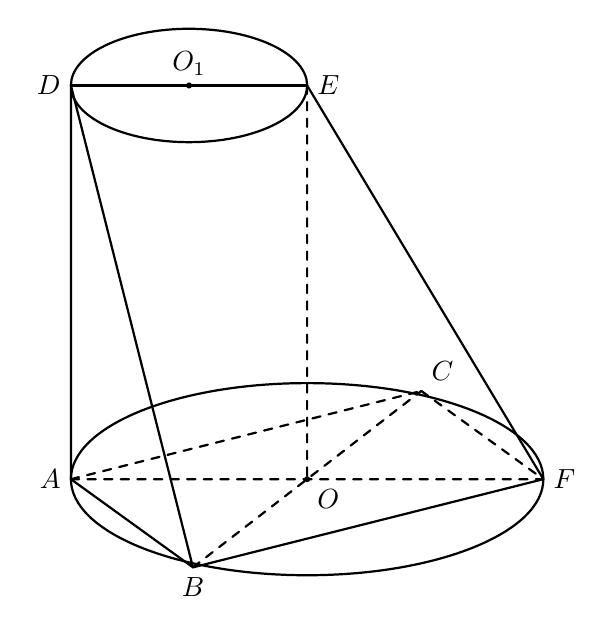
\begin{tikzpicture}[line cap=round,line join=round,thick]
  \coordinate (A) at (-3,0); \coordinate (F) at (3,0);
  \coordinate (B) at (-1.45,-1.12); \coordinate (C) at (1.45,1.12);
  \coordinate (O) at (0,0); \coordinate (D) at (-3,5.0);
  \coordinate (E) at (0,5.0); \coordinate (Oone) at (-1.5,5.0);
  % Circular rims and the upper diameter.
  \draw (0,0) ellipse (3 and 1.22);
  \draw (Oone) ellipse (1.5 and 0.72);
  \draw (D)--(E);
  % Solid spatial edges.
  \draw (A)--(D) (D)--(B) (E)--(F) (A)--(B)--(F);
  % Dashed diameter and internal construction edges from the source figure.
  \draw[dashed] (A)--(F) (E)--(O) (A)--(C) (C)--(F) (B)--(C) (B)--(O);
  \fill (O) circle (1.1pt); \fill (Oone) circle (1.1pt);
  \node[left] at (A) {$A$}; \node[below] at (B) {$B$};
  \node[above right] at (C) {$C$}; \node[right] at (F) {$F$};
  \node[left] at (D) {$D$}; \node[right] at (E) {$E$};
  \node[below right] at (O) {$O$}; \node[above] at (Oone) {$O_1$};
\end{tikzpicture}
